\item{
            \textbf{\enfr{ Feature Maps}{ Fonctions de transformation des données}}
            \points{10 points}{8 points}

            \enfr{
	            In this exercise, you will design feature maps to transform an original dataset into a linearly separable set of points. For the following questions, if your answer is `\textit{yes}', write the expression for the proposed transformation; and if your answer is `\textit{no}', write a brief explanation. You are expected to provide explicit formulas for the feature maps, and these formulas should only use common mathematical operations.
            }{
	            Dans cet exercice, vous allez concevoir des fonctions de transformation depuis l'espace de features original vers un espace où les données sont linéairement séparables. Pour les questions suivantes, si vous répondez `\textit{oui}', écrivez l'expression de la transformation correspondante; et si votre réponse est `\textit{non}', ajoutez une courte justification de votre réponse. Vous devez donner les formules explicites des transformations, et ces formules doivent utiliser uniquement des opérations mathématiques simples.
            }

            \begin{enumerate}
	            \item { [3 points] \enfr{
		                  Consider the following 1-D dataset (Figure \ref{a}). Can you propose a 1-D transformation that will make the points linearly separable?
	                  }{
		                  Soient les données 1-D suivantes (Figure \ref{a}). Pouvez-vous proposer une transformation 1-D (i.e. vers un espace de dimension 1) qui rend les points linéairement séparables?
	                  }

	                  \begin{figure}[!h]
		                  \centering
		                  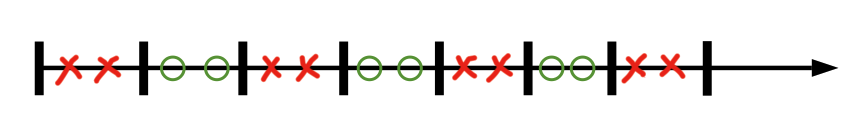
\includegraphics[width=0.55\textwidth]{img/Q2-a.png}
		                  \caption{\enfr{1-D dataset. The points between $2k$ and $2k+1$ are labeled by X. The points between $2k+1$ and $2k+2$ are labeled by O.}{Jeu de données 1D. Les points entre $2k$ et $2k+1$ sont étiquetés par X. Les points entre $2k+1$ et $2k+2$ sont étiquetés par O.}}
		                  \label{a}
	                  \end{figure}}
	                  %     \item {[2 points] In the same dataset, can you propose a 2-D transformation that makes the points linearly separable?}

	                  \begin{reponse}

		                  La transformation 1-D suivante sépare linéairement les points étiquetés par X et O :
		                  \begin{equation*}
			                  \phi(x) = \sin\left(\pi x\right)
		                  \end{equation*}
		                  $\phi(x) \geq 0$ lorsque $x \in$X et $\phi(x) < 0$ si $x \in$O
	                  \end{reponse}

	            \item { [3 points]
	                  \enfr{
		                  Consider the following 2-D dataset (Figure \ref{b}). Can you propose a transformation into 1-D that will make the data linearly separable?
	                  }{
		                  Soient les données 2-D suivantes (Figure \ref{b}). Pouvez-vous proposer une transformation 1-D qui rend les points linéairement séparables ?
	                  }
	                  \begin{figure}[h]
		                  \centerline{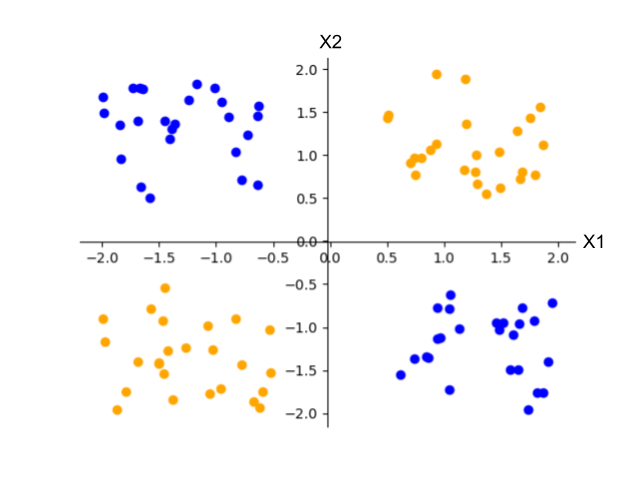
\includegraphics[scale=0.4]{img/Q2-b.png}}
		                  \caption{\enfr{2D dataset.}{Jeu de données 2D.}}
		                  \label{b}
	                  \end{figure}}

	                  \begin{reponse}

		                  La transformation 1-D suivante sépare linéairement les points bleus et orange :

		                  Soit $x\in \mathbb{R}^2$
		                  \begin{equation*}
			                  \phi\left(x\right)
			                  = \phi\left( \begin{bmatrix}
					                  x_1 \\
					                  x_2\end{bmatrix}\right) = x_1 x_2 \in \mathbb{R}
		                  \end{equation*}
		                  $\phi(x) \geq 0$ lorsque $x$ est un point appartenant à la classe orange et $\phi(x) < 0$ si $x$ est dans la classe bleue
	                  \end{reponse}

	            \item { [4 points]
	                  \enfr{
		                  Using ideas from the above two datasets, can you suggest a transformation of the following dataset (as shown in Figure \ref{12}) that makes it linearly separable? If `\textit{yes}', also provide the kernel corresponding to the feature map you proposed. Remember that $K(x, y)=\phi(x) \cdot \phi(y)$, so you can find $\phi$ and do the dot product to find an expression for the kernel.
	                  }{
		                  En utilisant les idées que vous avez utilisées pour les deux questions précédentes, pouvez-vous proposer une transformation des données suivantes (Figure \ref{12}) qui les rendent linéairement séparables? Si votre réponse est `\textit{oui}', donnez l'expression du noyau qui correspond à la transformation proposée. Souvenez-vous que $K(x, y)=\langle\phi(x) , \phi(y)\rangle$, donc trouvez $\phi$ et faites le produit scalaire pour obtenir le noyau.
	                  }
	                  \begin{figure}[H]
		                  \centering
		                  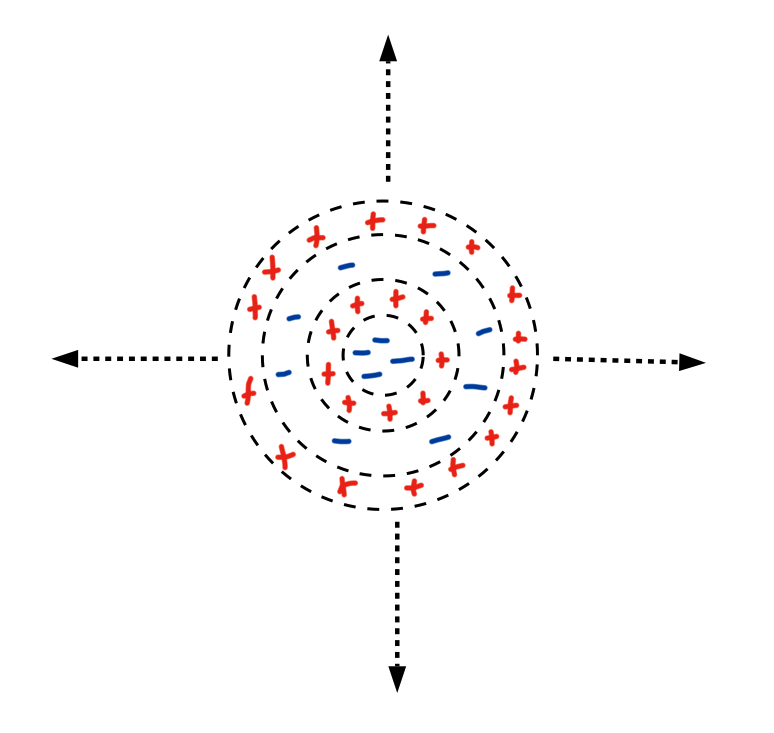
\includegraphics[scale=0.5]{img/Q2-c.png}
		                  \caption{\enfr{Another 2D dataset. The points between the areas of radius $2k$ and $2k+1$ are labeled by -. The points between the areas of radius $2k+1$ and $2k+2$ are labeled by +.}{Un autre jeu de données 2D. Les points entre les aires de rayon $2k$ et $2k+1$ sont étiquetés par -. Les points entre les aires de rayon $2k+1$ et $2k+2$ sont étiquetés par +.}}
		                  \label{12}
	                  \end{figure}}

	                  \begin{reponse}

		                  La transformation 3-D suivante sépare linéairement les points appartenant aux classes "+" et "-" selon le plan $z=0$

		                  Soit $x\in \mathbb{R}^2$
		                  \begin{equation*}
			                  \phi\left(x\right)
			                  = \phi\left( \begin{bmatrix}
					                  x_1 \\
					                  x_2\end{bmatrix}\right) = \begin{bmatrix}
				                  x_1 \\
				                  x_2 \\
				                  \sin\left(\pi {\lVert x \rVert}_2 \right)\end{bmatrix} \in \mathbb{R}^3
		                  \end{equation*}

		                  Déterminons maintenant le noyau :
		                  \begin{align*}
			                  K(x, y)
			                   & = \langle\phi(x),\phi(y)\rangle                                                                       \\
			                   & = x_1 y_1 + x_2 y_2 + \sin\left(\pi{\lVert x \rVert}_2\right)\sin\left(\pi{\lVert y \rVert}_2\right)  \\
			                   & = \langle x,y\rangle + \sin\left(\pi{\lVert x \rVert}_2\right)\sin\left(\pi{\lVert y \rVert}_2\right)
		                  \end{align*}

		                  \underline{Remarque :} On pourrait se contenter de la transformation 1-D : $\phi\left(x\right) = \sin\left(\pi {\lVert x \rVert}_2 \right)$
	                  \end{reponse}

            \end{enumerate}
      }
